In order to test the performance of the discrete controller, it has been implemented on the continuous time linear system (SIMULINK model figure \ref{fig:modelp16} in Appendix \ref{AppP16}).

As we can see figure \ref{fig:p16d0} and figure \ref{fig:p16d}, the controller works well, that is to say, the reference position is well followed. Indeed, with or without the noise \textbf{d}, the tracking is the same.

\begin{figure}[H]
 \centering 
 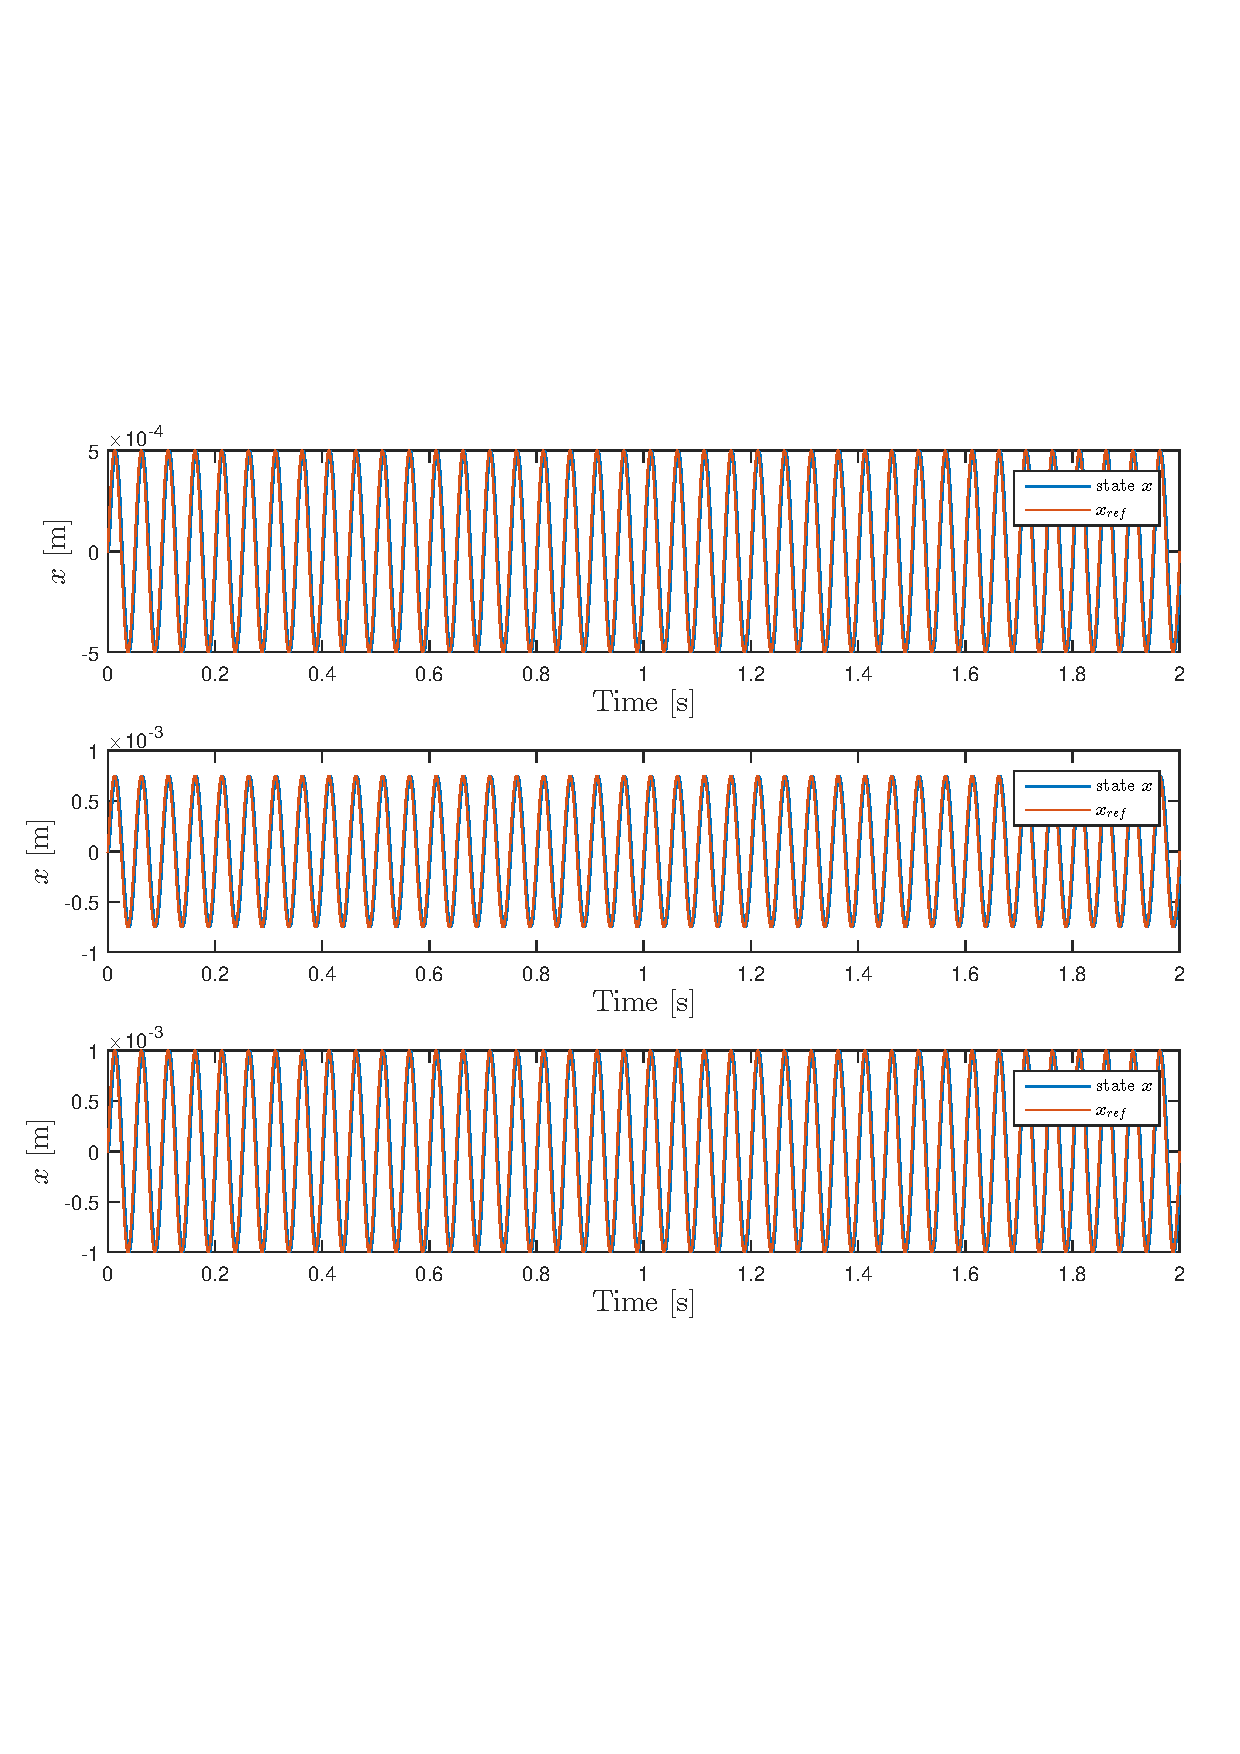
\includegraphics[trim=2cm 7cm 2cm 7cm, clip=true, totalheight=0.35\textheight, angle=0]{figures/p16d0.pdf}
 \caption{response of the state x to the input $x_{ref}$ with $Ax = 0.0005\ m$ and $f_c = 20\ Hz$ then $Ax = 0.001\ m$ and $f_c = 200\ Hz$ (from the top to the bottom) with the controller without disturbance}
 \label{fig:p16d0}
\end{figure}

\begin{figure}[H]
 \centering 
 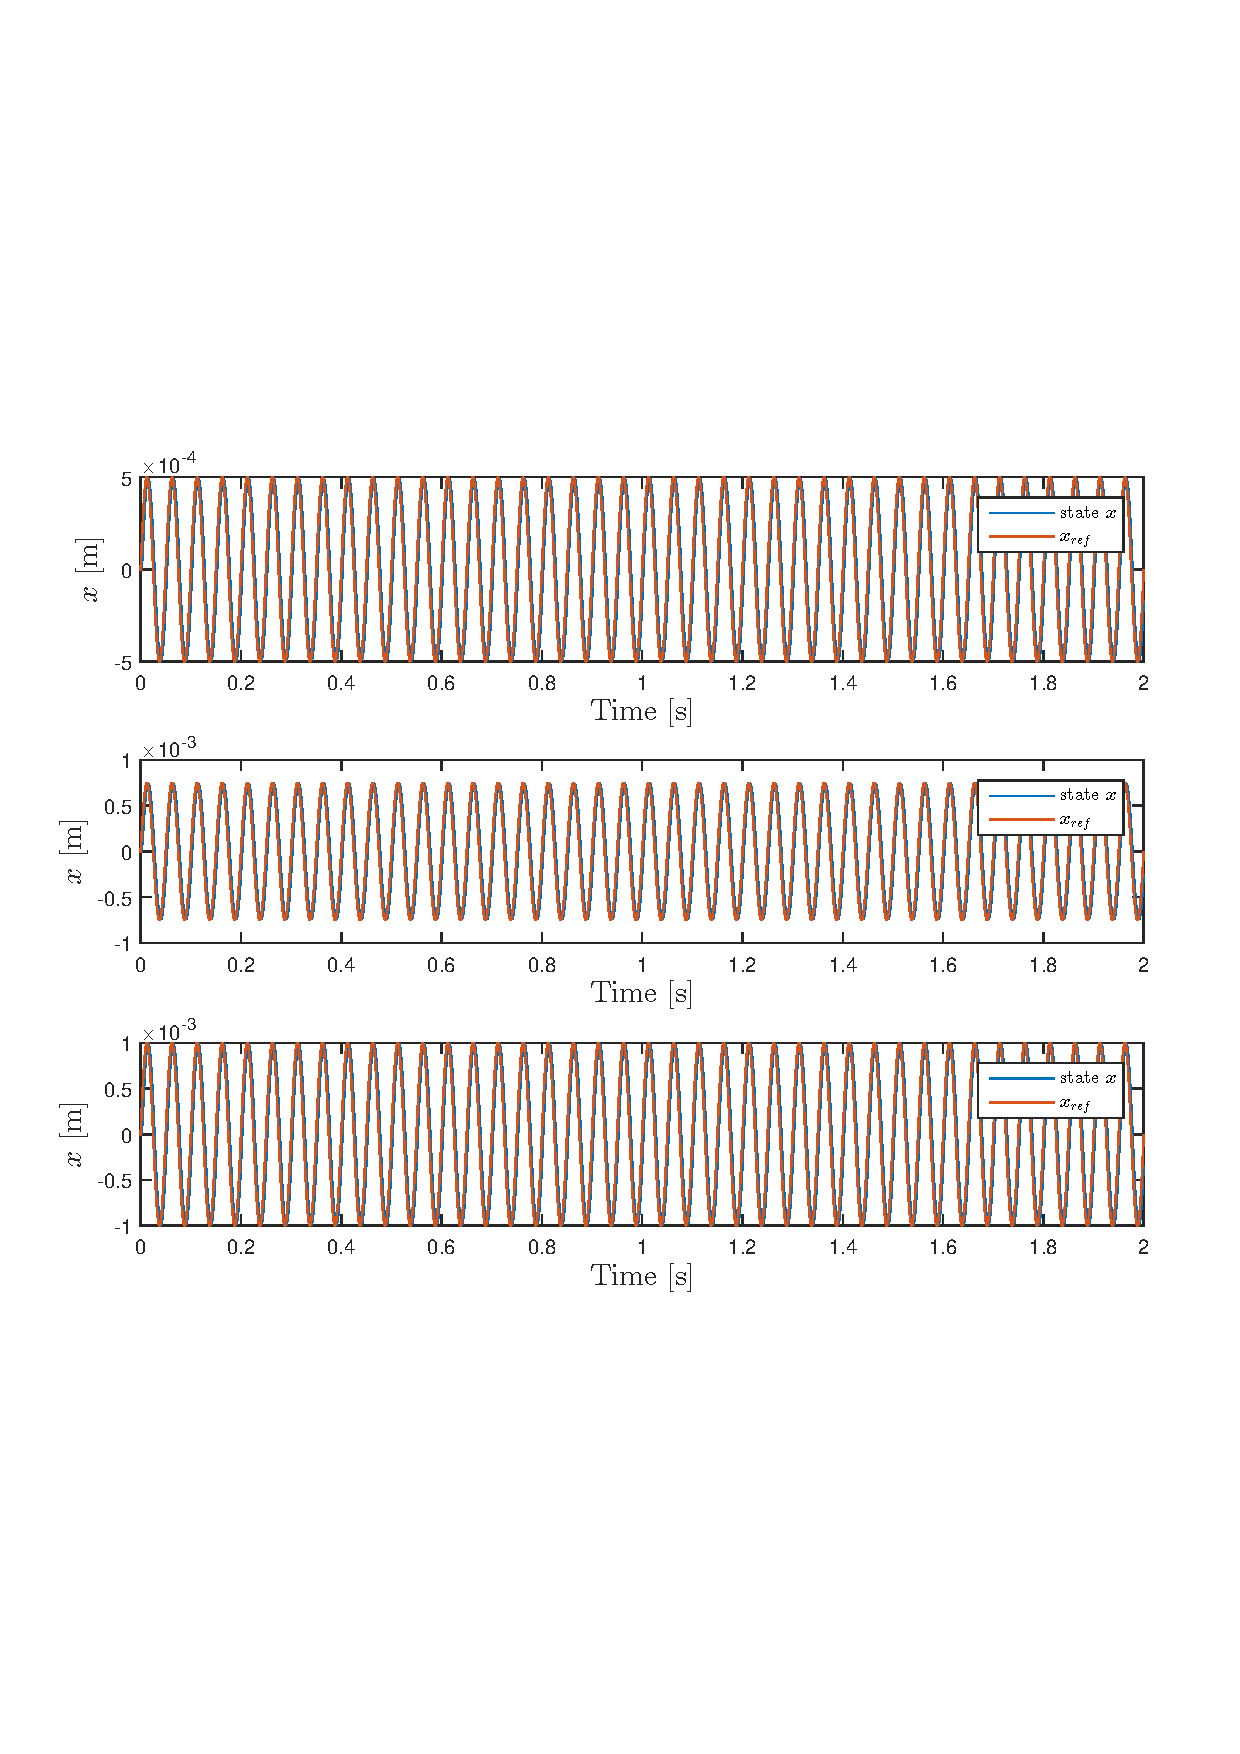
\includegraphics[trim=2cm 7cm 2cm 7cm, clip=true, totalheight=0.35\textheight, angle=0]{figures/p16d.pdf}
 \caption{response of the state x to the input $x_{ref} = x_{ln}$, the timeserie recorded in P9, with $f_c = 20\ Hz$ then $f_c=200\ Hz$ (from the top to the bottom) with the controller with the disturbance \textbf{d}}
 \label{fig:p16d}
\end{figure}

We can notice that it is odd that there is no difference between the simulation with or without the noise \textbf{d}.


Moreover, as we can see figure \ref{fig:p16ue}, in both case, we respect $u_e < 40\ V$.

\begin{figure}[H]
 \centering 
 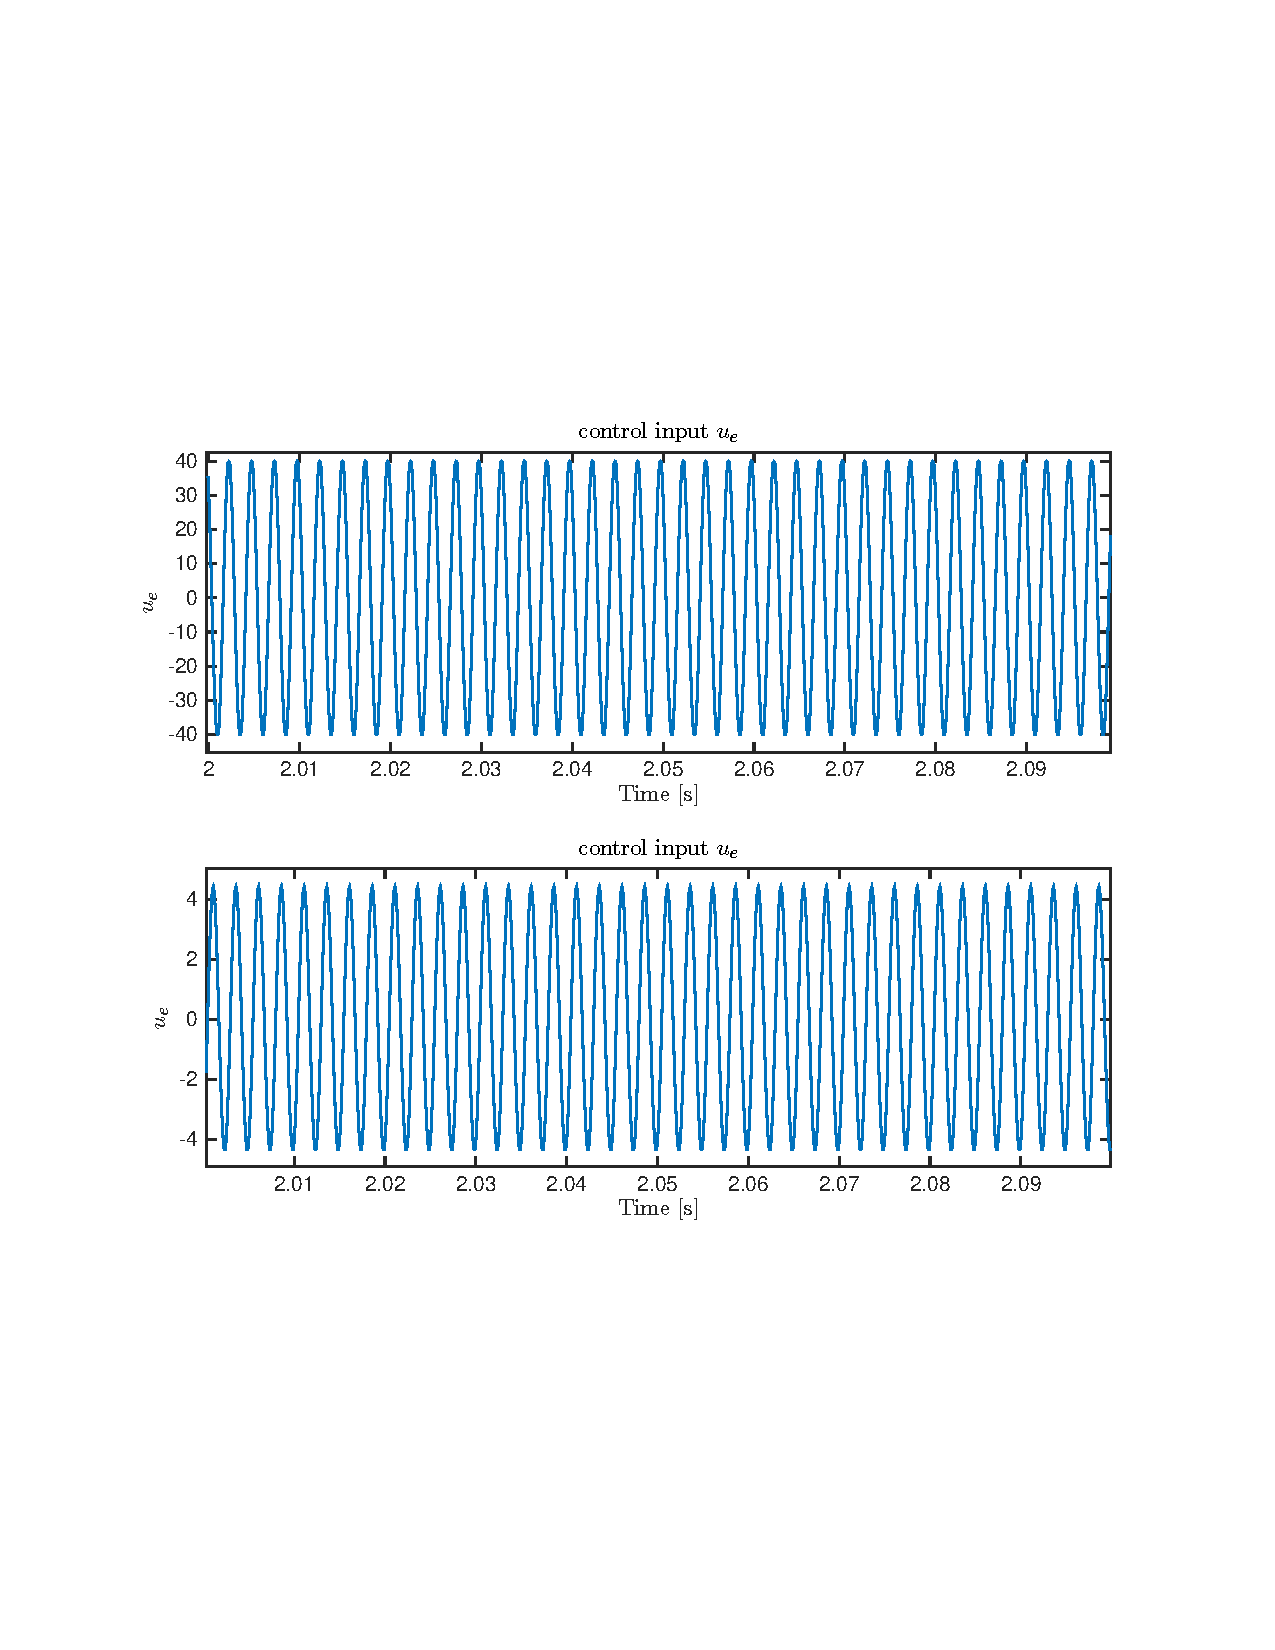
\includegraphics[trim=2cm 7cm 2cm 7cm, clip=true, totalheight=0.35\textheight, angle=0]{figures/p16ue.pdf}
 \caption{1. $u_e$ with an input $x_{ref}$ with $A_x=0.001\ m$ and $f_c = 200\ Hz$ with the controller without disturbance\\
2. $u_e$ with an input $x_{ref} = x_{ln}$ with $f_c = 200\ Hz$ with the controller and with disturbance \textbf{d}}
 \label{fig:p16ue}
\end{figure}
